% ============================================================
%  XOR gate - compact breadboard wiring diagram.
%  The native complementary (CMOS-style) XOR: 12 transistors on
%  ONE standard full-size 830-point breadboard (63 columns).
%      inverters: Q9/Q10 -> A-bar,  Q11/Q12 -> B-bar
%      pull-down (2N3904): Q1(A)+Q2(B) series  par  Q3(Abar)+Q4(Bbar) series
%      pull-up  (2N3906): Q5(A) par Q6(B),  in series (node u)
%                          with  Q7(Abar) par Q8(Bbar)
%  LEDs on the external inputs and output only.
%  Rail use:  top rail pair = +5 V (outer) and GND (inner) for
%  the transistor emitters; bottom rail = GND for the LED
%  returns.  ALL GND rails are ONE node - bridge them.
%  TO-92 legs sit in ADJACENT holes (E B C, left to right).
%  Compile:  pdflatex wiring.tex
% ============================================================
\documentclass[border=16pt]{standalone}
\usepackage{circuitikz}
\usepackage{tikz}
\usetikzlibrary{calc, positioning}

\definecolor{vcc}{RGB}{205,45,45}      % +5 V wires (red)
\definecolor{gnd}{RGB}{35,35,40}       % GND wires (near-black)
\definecolor{anet}{RGB}{20,140,60}     % input A (green)
\definecolor{bnet}{RGB}{225,120,0}     % input B (orange)
\definecolor{nanet}{RGB}{0,128,128}    % A-bar (teal)
\definecolor{nbnet}{RGB}{186,32,124}   % B-bar (magenta)
\definecolor{mnet}{RGB}{120,90,60}     % internal nodes m1, m2, u (brown)
\definecolor{onet}{RGB}{120,45,175}    % output (violet)
\definecolor{board}{RGB}{246,241,229}  % breadboard body

% one TO-92 transistor, legs in ADJACENT holes (dense build).
% #1 = column of the E leg, #2 = reference tag, #3 = part number
\newcommand{\transd}[3]{%
  \pgfmathsetmacro\xe{0.7*#1}%
  \pgfmathsetmacro\xb{0.7*(#1+1)}%
  \pgfmathsetmacro\xc{0.7*(#1+2)}%
  \draw[fill=black!10]
        (\xe-0.34,9.55) -- (\xe-0.34,9.9)
        arc (180:0:{(\xc-\xe+0.68)/2} and 0.42) -- (\xc+0.34,9.55) -- cycle;
  \node[font=\tiny\bfseries] at (\xb,10.04) {#2};
  \node[font=\tiny] at (\xb,9.76) {#3};
  \draw (\xe,9.55)--(\xe,9.0);
  \draw (\xb,9.55)--(\xb,9.0);
  \draw (\xc,9.55)--(\xc,9.0);
  \node[red,font=\tiny\bfseries,anchor=north] at (\xe,8.95) {E};
  \node[red,font=\tiny\bfseries,anchor=north] at (\xb,8.95) {B};
  \node[red,font=\tiny\bfseries,anchor=north] at (\xc,8.95) {C};
}

\begin{document}
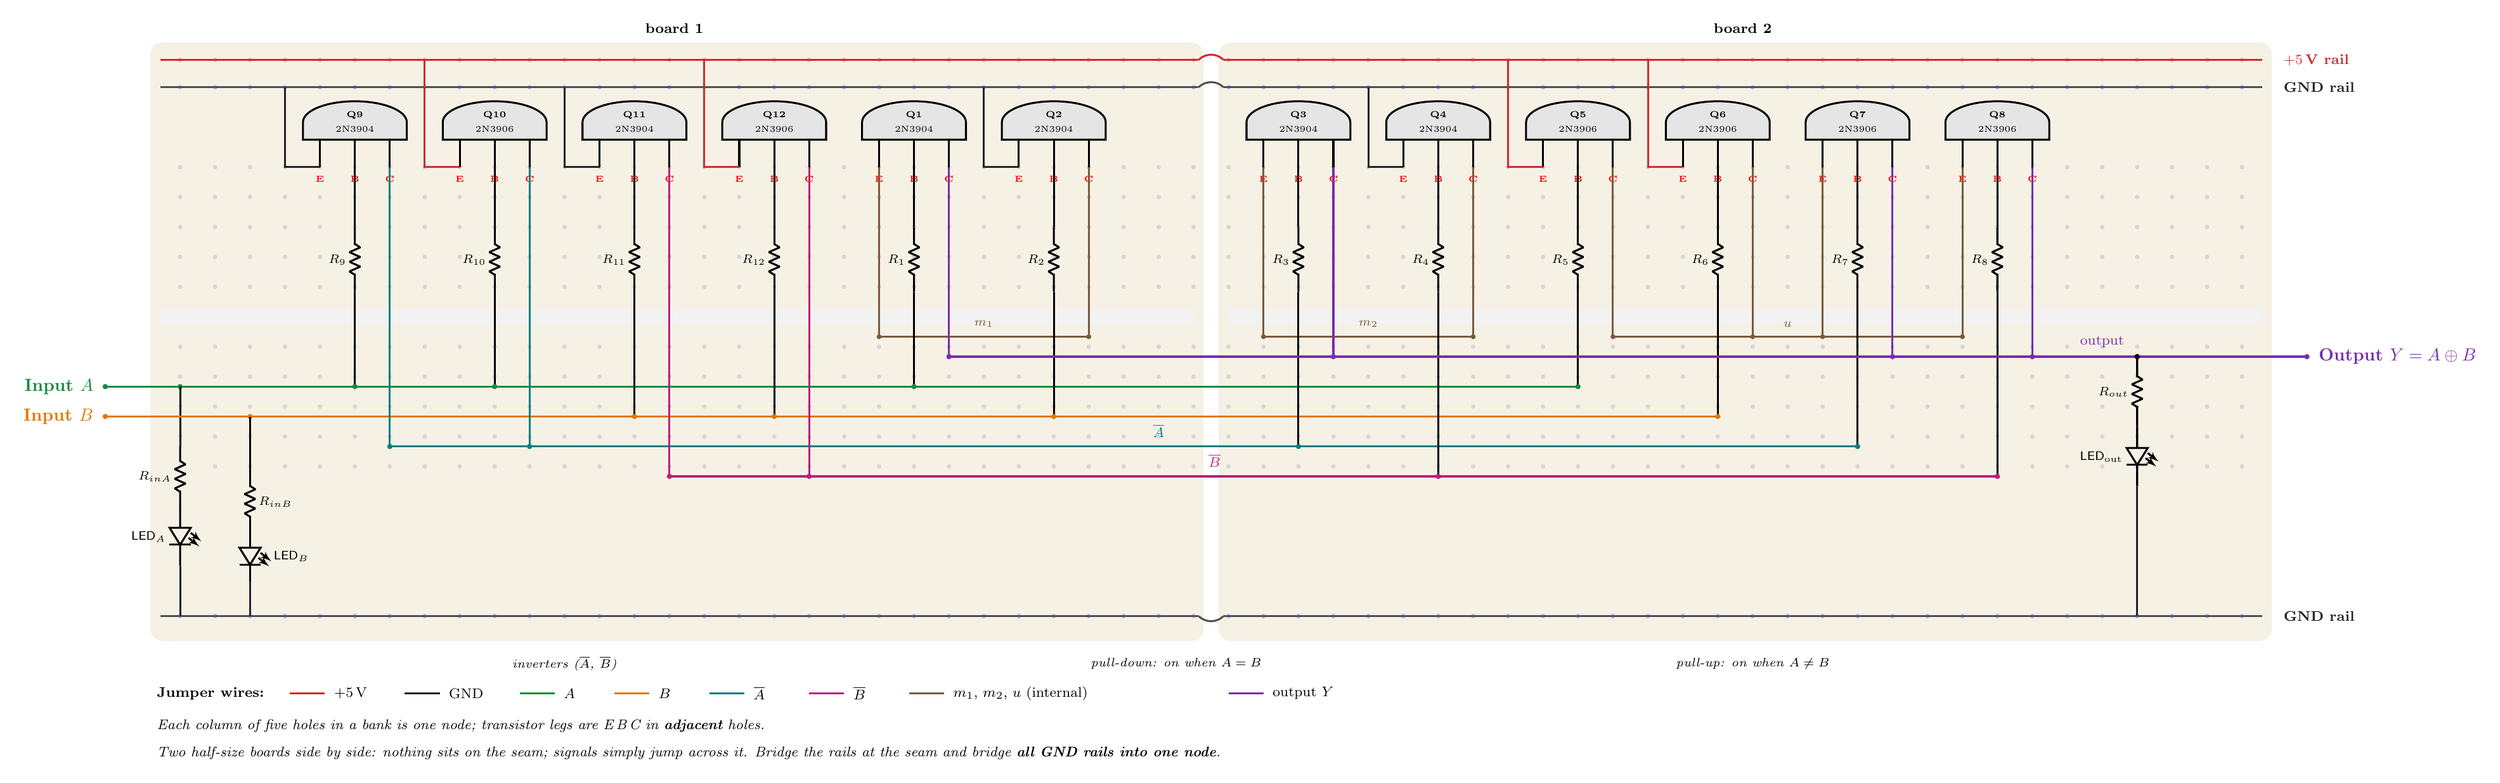
\begin{tikzpicture}[line width=1.1pt, font=\sffamily]
  \ctikzset{bipoles/thickness=1, bipoles/length=0.85cm, resistors/scale=0.85}

  % ---------- the two board bodies (abutted; seam between cols 30 / 31) ----------
  \fill[board,rounded corners=7pt] (0.1,-0.5)  rectangle (21.2,11.5);
  \fill[board,rounded corners=7pt] (21.5,-0.5) rectangle (42.6,11.5);
  \node[font=\footnotesize\bfseries,anchor=south] at (10.6,11.55) {board 1};
  \node[font=\footnotesize\bfseries,anchor=south] at (32.0,11.55) {board 2};

  % ---------- hole grid (two banks of 5 rows, both boards) ----------
  \foreach \c in {1,...,60}{
    \foreach \y in {9.0,8.4,7.8,7.2,6.6, 5.4,4.8,4.2,3.6,3.0}{
      \fill[black!16] ({0.7*\c},\y) circle (0.45mm);
    }
  }
  % centre gaps (ravines)
  \fill[black!5] (0.3,5.85)  rectangle (21.0,6.15);
  \fill[black!5] (21.7,5.85) rectangle (42.4,6.15);

  % ---------- power rails: top pair (+5 V outer, GND inner), bottom GND ----------
  \foreach \c in {1,...,60}{
    \fill[red!28]  ({0.7*\c},11.15) circle (0.45mm);
    \fill[blue!28] ({0.7*\c},10.6)  circle (0.45mm);
    \fill[blue!28] ({0.7*\c},0.0)   circle (0.45mm);
  }
  \draw[vcc]    (0.3,11.15)  -- (21.1,11.15);
  \draw[vcc]    (21.6,11.15) -- (42.4,11.15);
  \draw[gnd!80] (0.3,10.6)   -- (21.1,10.6);
  \draw[gnd!80] (21.6,10.6)  -- (42.4,10.6);
  \draw[gnd!80] (0.3,0.0)    -- (21.1,0.0);
  \draw[gnd!80] (21.6,0.0)   -- (42.4,0.0);
  % rail bridges across the seam
  \draw[vcc]    (21.1,11.15) to[bend left=45] (21.6,11.15);
  \draw[gnd!80] (21.1,10.6)  to[bend left=45] (21.6,10.6);
  \draw[gnd!80] (21.1,0.0)   to[bend right=45] (21.6,0.0);
  \node[vcc,font=\footnotesize\bfseries,anchor=west] at (42.7,11.15) {$+5\,$V rail};
  \node[gnd,font=\footnotesize\bfseries,anchor=west] at (42.7,10.6)  {GND rail};
  \node[gnd,font=\footnotesize\bfseries,anchor=west] at (42.7,0.0)   {GND rail};

  % ---------- transistors (legs E B C in adjacent holes) ----------
  \transd{5}{Q9}{2N3904}
  \transd{9}{Q10}{2N3906}
  \transd{13}{Q11}{2N3904}
  \transd{17}{Q12}{2N3906}
  \transd{21}{Q1}{2N3904}
  \transd{25}{Q2}{2N3904}
  \transd{32}{Q3}{2N3904}
  \transd{36}{Q4}{2N3904}
  \transd{40}{Q5}{2N3906}
  \transd{44}{Q6}{2N3906}
  \transd{48}{Q7}{2N3906}
  \transd{52}{Q8}{2N3906}

  % =========================================================
  %  emitters:  NPN -> top GND rail,  PNP -> +5 V rail
  %  (each jogs one column left, then straight up; Q1.E -> m1,
  %   Q3.E -> m2, Q7.E and Q8.E -> node u instead)
  % =========================================================
  \draw[gnd] ({0.7*5},9.0)  -- ({0.7*4},9.0)  -- ({0.7*4},10.6);    % Q9.E
  \draw[vcc] ({0.7*9},9.0)  -- ({0.7*8},9.0)  -- ({0.7*8},11.15);   % Q10.E
  \draw[gnd] ({0.7*13},9.0) -- ({0.7*12},9.0) -- ({0.7*12},10.6);   % Q11.E
  \draw[vcc] ({0.7*17},9.0) -- ({0.7*16},9.0) -- ({0.7*16},11.15);  % Q12.E
  \draw[gnd] ({0.7*25},9.0) -- ({0.7*24},9.0) -- ({0.7*24},10.6);   % Q2.E
  \draw[gnd] ({0.7*36},9.0) -- ({0.7*35},9.0) -- ({0.7*35},10.6);   % Q4.E
  \draw[vcc] ({0.7*40},9.0) -- ({0.7*39},9.0) -- ({0.7*39},11.15);  % Q5.E
  \draw[vcc] ({0.7*44},9.0) -- ({0.7*43},9.0) -- ({0.7*43},11.15);  % Q6.E

  % =========================================================
  %  series links (brown, y=5.6):
  %  m1: Q1.E (21) <-> Q2.C (27);   m2: Q3.E (32) <-> Q4.C (38)
  %  u : Q5.C (42) + Q6.C (46) <-> Q7.E (48) + Q8.E (52)
  % =========================================================
  \draw[mnet] ({0.7*21},9.0) -- ({0.7*21},5.6);
  \draw[mnet] ({0.7*27},9.0) -- ({0.7*27},5.6);
  \draw[mnet] ({0.7*21},5.6) -- ({0.7*27},5.6);
  \fill[mnet] ({0.7*21},5.6) circle (1.4pt); \fill[mnet] ({0.7*27},5.6) circle (1.4pt);
  \node[mnet,font=\scriptsize,anchor=south] at ({0.7*24},5.65) {$m_1$};

  \draw[mnet] ({0.7*32},9.0) -- ({0.7*32},5.6);
  \draw[mnet] ({0.7*38},9.0) -- ({0.7*38},5.6);
  \draw[mnet] ({0.7*32},5.6) -- ({0.7*38},5.6);
  \fill[mnet] ({0.7*32},5.6) circle (1.4pt); \fill[mnet] ({0.7*38},5.6) circle (1.4pt);
  \node[mnet,font=\scriptsize,anchor=south] at ({0.7*35},5.65) {$m_2$};

  \draw[mnet] ({0.7*42},9.0) -- ({0.7*42},5.6);
  \draw[mnet] ({0.7*46},9.0) -- ({0.7*46},5.6);
  \draw[mnet] ({0.7*48},9.0) -- ({0.7*48},5.6);
  \draw[mnet] ({0.7*52},9.0) -- ({0.7*52},5.6);
  \draw[mnet] ({0.7*42},5.6) -- ({0.7*52},5.6);
  \fill[mnet] ({0.7*42},5.6) circle (1.4pt); \fill[mnet] ({0.7*46},5.6) circle (1.4pt);
  \fill[mnet] ({0.7*48},5.6) circle (1.4pt); \fill[mnet] ({0.7*52},5.6) circle (1.4pt);
  \node[mnet,font=\scriptsize,anchor=south] at ({0.7*47},5.65) {$u$};

  % =========================================================
  %  INPUT A net (green), lane at y=4.6:
  %  terminal -> R9 (Q9.B, col6) -> R10 (Q10.B, col10)
  %           -> R1 (Q1.B, col22) -> R5 (Q5.B, col41); LED on col1
  % =========================================================
  \draw[anet] (-0.8,4.6) -- ({0.7*41},4.6);
  \node[anet,anchor=east,font=\bfseries] at (-0.9,4.6) {Input $A$};
  \fill[anet] (-0.8,4.6) circle (1.5pt);
  \foreach \col/\rlab in {6/{R_{9}}, 10/{R_{10}}, 22/{R_{1}}, 41/{R_{5}}}{
    \draw ({0.7*\col},9.0) -- ({0.7*\col},7.8);
    \draw ({0.7*\col},7.8) to[R, l_=\scriptsize $\rlab$] ({0.7*\col},6.5);
    \draw ({0.7*\col},6.5) -- ({0.7*\col},4.6);
    \fill[anet] ({0.7*\col},4.6) circle (1.5pt);
  }
  % input indicator LED on col 1
  \fill[anet] ({0.7*1},4.6) circle (1.5pt);
  \draw ({0.7*1},4.6) -- ({0.7*1},3.4);
  \draw ({0.7*1},3.4) to[R, l_=\scriptsize $R_{inA}$] ({0.7*1},2.2);
  \draw ({0.7*1},2.2) to[leD, l_=\scriptsize LED$_A$] ({0.7*1},1.0);
  \draw[gnd] ({0.7*1},1.0) -- ({0.7*1},0.0);

  % =========================================================
  %  INPUT B net (orange), lane at y=4.0:
  %  terminal -> R11 (Q11.B, col14) -> R12 (Q12.B, col18)
  %           -> R2 (Q2.B, col26) -> R6 (Q6.B, col45); LED on col3
  % =========================================================
  \draw[bnet] (-0.8,4.0) -- ({0.7*45},4.0);
  \node[bnet,anchor=east,font=\bfseries] at (-0.9,4.0) {Input $B$};
  \fill[bnet] (-0.8,4.0) circle (1.5pt);
  \foreach \col/\rlab in {14/{R_{11}}, 18/{R_{12}}, 26/{R_{2}}, 45/{R_{6}}}{
    \draw ({0.7*\col},9.0) -- ({0.7*\col},7.8);
    \draw ({0.7*\col},7.8) to[R, l_=\scriptsize $\rlab$] ({0.7*\col},6.5);
    \draw ({0.7*\col},6.5) -- ({0.7*\col},4.0);
    \fill[bnet] ({0.7*\col},4.0) circle (1.5pt);
  }
  % input indicator LED on col 3
  \fill[bnet] ({0.7*3},4.0) circle (1.5pt);
  \draw ({0.7*3},4.0) -- ({0.7*3},2.9);
  \draw ({0.7*3},2.9) to[R, l=\scriptsize $R_{inB}$] ({0.7*3},1.7);
  \draw ({0.7*3},1.7) to[leD, l=\scriptsize LED$_B$] ({0.7*3},0.7);
  \draw[gnd] ({0.7*3},0.7) -- ({0.7*3},0.0);

  % =========================================================
  %  A-bar net (teal), lane at y=3.4:
  %  Q9.C (7) + Q10.C (11)  ->  R3 (Q3.B, col33) + R7 (Q7.B, col49)
  % =========================================================
  \draw[nanet] ({0.7*7},9.0)  -- ({0.7*7},3.4);
  \draw[nanet] ({0.7*11},9.0) -- ({0.7*11},3.4);
  \draw[nanet] ({0.7*7},3.4)  -- ({0.7*49},3.4);
  \fill[nanet] ({0.7*7},3.4)  circle (1.5pt);
  \fill[nanet] ({0.7*11},3.4) circle (1.5pt);
  \node[nanet,font=\footnotesize,anchor=south] at ({0.7*29},3.45) {$\overline{A}$};
  \foreach \col/\rlab in {33/{R_{3}}, 49/{R_{7}}}{
    \draw ({0.7*\col},9.0) -- ({0.7*\col},7.8);
    \draw ({0.7*\col},7.8) to[R, l_=\scriptsize $\rlab$] ({0.7*\col},6.5);
    \draw ({0.7*\col},6.5) -- ({0.7*\col},3.4);
    \fill[nanet] ({0.7*\col},3.4) circle (1.5pt);
  }

  % =========================================================
  %  B-bar net (magenta), lane at y=2.8:
  %  Q11.C (15) + Q12.C (19)  ->  R4 (Q4.B, col37) + R8 (Q8.B, col53)
  % =========================================================
  \draw[nbnet] ({0.7*15},9.0) -- ({0.7*15},2.8);
  \draw[nbnet] ({0.7*19},9.0) -- ({0.7*19},2.8);
  \draw[nbnet] ({0.7*15},2.8) -- ({0.7*53},2.8);
  \fill[nbnet] ({0.7*15},2.8) circle (1.5pt);
  \fill[nbnet] ({0.7*19},2.8) circle (1.5pt);
  \node[nbnet,font=\footnotesize,anchor=south] at ({0.7*30.6},2.85) {$\overline{B}$};
  \foreach \col/\rlab in {37/{R_{4}}, 53/{R_{8}}}{
    \draw ({0.7*\col},9.0) -- ({0.7*\col},7.8);
    \draw ({0.7*\col},7.8) to[R, l_=\scriptsize $\rlab$] ({0.7*\col},6.5);
    \draw ({0.7*\col},6.5) -- ({0.7*\col},2.8);
    \fill[nbnet] ({0.7*\col},2.8) circle (1.5pt);
  }

  % =========================================================
  %  OUTPUT net (violet), lane at y=5.2:
  %  Q1.C (23) + Q3.C (34) + Q7.C (50) + Q8.C (54)
  %      -> LED (col57) -> terminal
  % =========================================================
  \draw[onet] ({0.7*23},9.0) -- ({0.7*23},5.2);
  \draw[onet] ({0.7*34},9.0) -- ({0.7*34},5.2);
  \draw[onet] ({0.7*50},9.0) -- ({0.7*50},5.2);
  \draw[onet] ({0.7*54},9.0) -- ({0.7*54},5.2);
  \draw[onet] ({0.7*23},5.2) -- (43.3,5.2);
  \fill[onet] ({0.7*23},5.2) circle (1.5pt);
  \fill[onet] ({0.7*34},5.2) circle (1.5pt);
  \fill[onet] ({0.7*50},5.2) circle (1.5pt);
  \fill[onet] ({0.7*54},5.2) circle (1.5pt);
  \node[onet,font=\footnotesize,anchor=south] at ({0.7*56},5.25) {output};
  \node[onet,anchor=west,font=\bfseries] at (43.4,5.2) {Output $Y=A\oplus B$};
  \fill[onet] (43.3,5.2) circle (1.5pt);
  % output indicator LED on col 57
  \draw ({0.7*57},5.2) to[R, l_=\scriptsize $R_{out}$, *-] ({0.7*57},3.8);
  \draw ({0.7*57},3.8) to[leD, l_=\scriptsize LED$_{\mathrm{out}}$] ({0.7*57},2.6);
  \draw[gnd] ({0.7*57},2.6) -- ({0.7*57},0.0);

  % =========================================================
  %  section tags
  % =========================================================
  \node[font=\scriptsize\itshape,anchor=south] at ({0.7*12},10.55) {};
  \node[font=\scriptsize\itshape] at ({0.7*12},-0.95) {inverters ($\overline{A}$, $\overline{B}$)};
  \node[font=\scriptsize\itshape] at ({0.7*29.5},-0.95) {pull-down: on when $A=B$};
  \node[font=\scriptsize\itshape] at ({0.7*46},-0.95) {pull-up: on when $A\neq B$};

  % =========================================================
  %  legend
  % =========================================================
  \begin{scope}[shift={(0.3,-2.1)}]
    \node[anchor=west,font=\footnotesize\bfseries] at (-0.2,0.55) {Jumper wires:};
    \draw[vcc]   (2.6,0.55)--(3.3,0.55);   \node[anchor=west,font=\footnotesize] at (3.35,0.55){+5\,V};
    \draw[gnd]   (4.9,0.55)--(5.6,0.55);   \node[anchor=west,font=\footnotesize] at (5.65,0.55){GND};
    \draw[anet]  (7.2,0.55)--(7.9,0.55);   \node[anchor=west,font=\footnotesize] at (7.95,0.55){$A$};
    \draw[bnet]  (9.1,0.55)--(9.8,0.55);   \node[anchor=west,font=\footnotesize] at (9.85,0.55){$B$};
    \draw[nanet] (11.0,0.55)--(11.7,0.55); \node[anchor=west,font=\footnotesize] at (11.75,0.55){$\overline{A}$};
    \draw[nbnet] (13.0,0.55)--(13.7,0.55); \node[anchor=west,font=\footnotesize] at (13.75,0.55){$\overline{B}$};
    \draw[mnet]  (15.0,0.55)--(15.7,0.55); \node[anchor=west,font=\footnotesize] at (15.75,0.55){$m_1$, $m_2$, $u$ (internal)};
    \draw[onet]  (21.4,0.55)--(22.1,0.55); \node[anchor=west,font=\footnotesize] at (22.15,0.55){output $Y$};
    \node[anchor=west,font=\footnotesize\itshape] at (-0.2,-0.1)
        {Each column of five holes in a bank is one node; transistor legs are E\,B\,C in \textbf{adjacent} holes.};
    \node[anchor=west,font=\footnotesize\itshape] at (-0.2,-0.65)
        {Two half-size boards side by side: nothing sits on the seam; signals simply jump across it.
         Bridge the rails at the seam and bridge \textbf{all GND rails into one node}.};
  \end{scope}

\end{tikzpicture}
\end{document}
